\documentclass[1p]{elsarticle_modified}
%\bibliographystyle{elsarticle-num}

%\usepackage[colorlinks]{hyperref}
%\usepackage{abbrmath_seonhwa} %\Abb, \Ascr, \Acal ,\Abf, \Afrak
\usepackage{amsfonts}
\usepackage{amssymb}
\usepackage{amsmath}
\usepackage{amsthm}
\usepackage{scalefnt}
\usepackage{amsbsy}
\usepackage{kotex}
\usepackage{caption}
\usepackage{subfig}
\usepackage{color}
\usepackage{graphicx}
\usepackage{xcolor} %% white, black, red, green, blue, cyan, magenta, yellow
\usepackage{float}
\usepackage{setspace}
\usepackage{hyperref}

\usepackage{tikz}
\usetikzlibrary{arrows}

\usepackage{multirow}
\usepackage{array} % fixed length table
\usepackage{hhline}

%%%%%%%%%%%%%%%%%%%%%
\makeatletter
\renewcommand*\env@matrix[1][\arraystretch]{%
	\edef\arraystretch{#1}%
	\hskip -\arraycolsep
	\let\@ifnextchar\new@ifnextchar
	\array{*\c@MaxMatrixCols c}}
\makeatother %https://tex.stackexchange.com/questions/14071/how-can-i-increase-the-line-spacing-in-a-matrix
%%%%%%%%%%%%%%%

\usepackage[normalem]{ulem}

\newcommand{\msout}[1]{\ifmmode\text{\sout{\ensuremath{#1}}}\else\sout{#1}\fi}
%SOURCE: \msout is \stkout macro in https://tex.stackexchange.com/questions/20609/strikeout-in-math-mode

\newcommand{\cancel}[1]{
	\ifmmode
	{\color{red}\msout{#1}}
	\else
	{\color{red}\sout{#1}}
	\fi
}

\newcommand{\add}[1]{
	{\color{blue}\uwave{#1}}
}

\newcommand{\replace}[2]{
	\ifmmode
	{\color{red}\msout{#1}}{\color{blue}\uwave{#2}}
	\else
	{\color{red}\sout{#1}}{\color{blue}\uwave{#2}}
	\fi
}

\newcommand{\Sol}{\mathcal{S}} %segment
\newcommand{\D}{D} %diagram
\newcommand{\A}{\mathcal{A}} %arc


%%%%%%%%%%%%%%%%%%%%%%%%%%%%%5 test

\def\sl{\operatorname{\textup{SL}}(2,\Cbb)}
\def\psl{\operatorname{\textup{PSL}}(2,\Cbb)}
\def\quan{\mkern 1mu \triangleright \mkern 1mu}

\theoremstyle{definition}
\newtheorem{thm}{Theorem}[section]
\newtheorem{prop}[thm]{Proposition}
\newtheorem{lem}[thm]{Lemma}
\newtheorem{ques}[thm]{Question}
\newtheorem{cor}[thm]{Corollary}
\newtheorem{defn}[thm]{Definition}
\newtheorem{exam}[thm]{Example}
\newtheorem{rmk}[thm]{Remark}
\newtheorem{alg}[thm]{Algorithm}

\newcommand{\I}{\sqrt{-1}}
\begin{document}

%\begin{frontmatter}
%
%\title{Boundary parabolic representations of knots up to 8 crossings}
%
%%% Group authors per affiliation:
%\author{Yunhi Cho} 
%\address{Department of Mathematics, University of Seoul, Seoul, Korea}
%\ead{yhcho@uos.ac.kr}
%
%
%\author{Seonhwa Kim} %\fnref{s_kim}}
%\address{Center for Geometry and Physics, Institute for Basic Science, Pohang, 37673, Korea}
%\ead{ryeona17@ibs.re.kr}
%
%\author{Hyuk Kim}
%\address{Department of Mathematical Sciences, Seoul National University, Seoul 08826, Korea}
%\ead{hyukkim@snu.ac.kr}
%
%\author{Seokbeom Yoon}
%\address{Department of Mathematical Sciences, Seoul National University, Seoul, 08826,  Korea}
%\ead{sbyoon15@snu.ac.kr}
%
%\begin{abstract}
%We find all boundary parabolic representation of knots up to 8 crossings.
%
%\end{abstract}
%\begin{keyword}
%    \MSC[2010] 57M25 
%\end{keyword}
%
%\end{frontmatter}

%\linenumbers
%\tableofcontents
%
\newcommand\colored[1]{\textcolor{white}{\rule[-0.35ex]{0.8em}{1.4ex}}\kern-0.8em\color{red} #1}%
%\newcommand\colored[1]{\textcolor{white}{ #1}\kern-2.17ex	\textcolor{white}{ #1}\kern-1.81ex	\textcolor{white}{ #1}\kern-2.15ex\color{red}#1	}

{\Large $\underline{11n_{86}~(K11n_{86})}$}

\setlength{\tabcolsep}{10pt}
\renewcommand{\arraystretch}{1.6}
\vspace{1cm}\begin{tabular}{m{100pt}>{\centering\arraybackslash}m{274pt}}
\multirow{5}{120pt}{
	\centering
	\includegraphics[width=112pt]{../../../GIT/diagram.site/Diagrams/png/702_11n_86.png}\\
\ \ \ A knot diagram\footnotemark}&
\allowdisplaybreaks
\textbf{Linearized knot diagam} \\
\cline{2-2}
 &
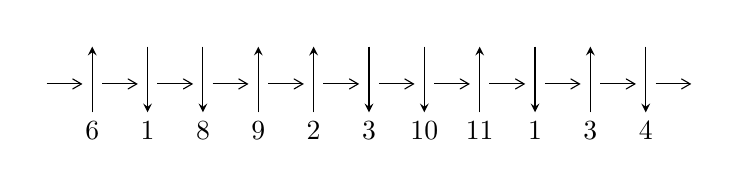
\begin{tikzpicture}[x=20pt, y=17pt]
	% nodes
	\node (C0) at (0, 0) {};
	\node (C1) at (1, 0) {};
	\node (C1U) at (1, +1) {};
	\node (C1D) at (1, -1) {6};

	\node (C2) at (2, 0) {};
	\node (C2U) at (2, +1) {};
	\node (C2D) at (2, -1) {1};

	\node (C3) at (3, 0) {};
	\node (C3U) at (3, +1) {};
	\node (C3D) at (3, -1) {8};

	\node (C4) at (4, 0) {};
	\node (C4U) at (4, +1) {};
	\node (C4D) at (4, -1) {9};

	\node (C5) at (5, 0) {};
	\node (C5U) at (5, +1) {};
	\node (C5D) at (5, -1) {2};

	\node (C6) at (6, 0) {};
	\node (C6U) at (6, +1) {};
	\node (C6D) at (6, -1) {3};

	\node (C7) at (7, 0) {};
	\node (C7U) at (7, +1) {};
	\node (C7D) at (7, -1) {10};

	\node (C8) at (8, 0) {};
	\node (C8U) at (8, +1) {};
	\node (C8D) at (8, -1) {11};

	\node (C9) at (9, 0) {};
	\node (C9U) at (9, +1) {};
	\node (C9D) at (9, -1) {1};

	\node (C10) at (10, 0) {};
	\node (C10U) at (10, +1) {};
	\node (C10D) at (10, -1) {3};

	\node (C11) at (11, 0) {};
	\node (C11U) at (11, +1) {};
	\node (C11D) at (11, -1) {4};
	\node (C12) at (12, 0) {};

	% arrows
	\draw[->,>={angle 60}]
	(C0) edge (C1) (C1) edge (C2) (C2) edge (C3) (C3) edge (C4) (C4) edge (C5) (C5) edge (C6) (C6) edge (C7) (C7) edge (C8) (C8) edge (C9) (C9) edge (C10) (C10) edge (C11) (C11) edge (C12) ;	\draw[->,>=stealth]
	(C1D) edge (C1U) (C2U) edge (C2D) (C3U) edge (C3D) (C4D) edge (C4U) (C5D) edge (C5U) (C6U) edge (C6D) (C7U) edge (C7D) (C8D) edge (C8U) (C9U) edge (C9D) (C10D) edge (C10U) (C11U) edge (C11D) ;
	\end{tikzpicture} \\
\hhline{~~} \\& 
\textbf{Solving Sequence} \\ \cline{2-2} 
 &
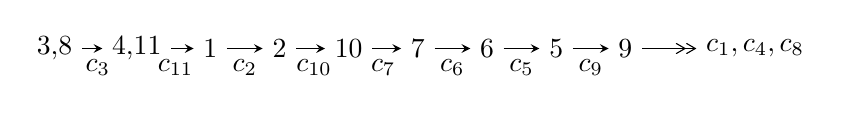
\begin{tikzpicture}[x=25pt, y=7pt]
	% node
	\node (A0) at (-1/8, 0) {3,8};
	\node (A1) at (17/16, 0) {4,11};
	\node (A2) at (17/8, 0) {1};
	\node (A3) at (25/8, 0) {2};
	\node (A4) at (33/8, 0) {10};
	\node (A5) at (41/8, 0) {7};
	\node (A6) at (49/8, 0) {6};
	\node (A7) at (57/8, 0) {5};
	\node (A8) at (65/8, 0) {9};
	\node (C1) at (1/2, -1) {$c_{3}$};
	\node (C2) at (13/8, -1) {$c_{11}$};
	\node (C3) at (21/8, -1) {$c_{2}$};
	\node (C4) at (29/8, -1) {$c_{10}$};
	\node (C5) at (37/8, -1) {$c_{7}$};
	\node (C6) at (45/8, -1) {$c_{6}$};
	\node (C7) at (53/8, -1) {$c_{5}$};
	\node (C8) at (61/8, -1) {$c_{9}$};
	\node (A9) at (10, 0) {$c_{1},c_{4},c_{8}$};

	% edge
	\draw[->,>=stealth]	
	(A0) edge (A1) (A1) edge (A2) (A2) edge (A3) (A3) edge (A4) (A4) edge (A5) (A5) edge (A6) (A6) edge (A7) (A7) edge (A8) ;
	\draw[->>,>={angle 60}]	
	(A8) edge (A9);
\end{tikzpicture} \\ 

\end{tabular} \\

\footnotetext{
The image of knot diagram is generated by the software ``\textbf{Draw programme}" developed by Andrew Bartholomew(\url{http://www.layer8.co.uk/maths/draw/index.htm\#Running-draw}), where we modified some parts for our purpose(\url{https://github.com/CATsTAILs/LinksPainter}).
}\phantom \\ \newline 
\centering \textbf{Ideals for irreducible components\footnotemark of $X_{\text{par}}$} 
 
\begin{align*}
I^u_{1}&=\langle 
-43 u^9+25 u^8+66 u^7-10 u^6-255 u^5+76 u^4+202 u^3+72 u^2+77 b-63 u-107,\\
\phantom{I^u_{1}}&\phantom{= \langle  }-200 u^9+93 u^8+264 u^7-68 u^6-1041 u^5+255 u^4+773 u^3+197 u^2+77 a-105 u-435,\\
\phantom{I^u_{1}}&\phantom{= \langle  }u^{10}- u^9- u^8+u^7+5 u^6-4 u^5-3 u^4+u^3+u^2+2 u-1\rangle \\
I^u_{2}&=\langle 
- u^4+u^2+b- u-1,\;-3 u^4- u^3+2 u^2+a-2 u-3,\;u^5- u^3+u^2+u-1\rangle \\
I^u_{3}&=\langle 
624 u^{13}+464 u^{12}+\cdots+481 b-103,\;879 u^{13}+406 u^{12}+\cdots+481 a-2102,\\
\phantom{I^u_{3}}&\phantom{= \langle  }u^{14}+6 u^{10}- u^9- u^8-4 u^7+12 u^6-4 u^5+5 u^4-10 u^3+11 u^2-5 u+1\rangle \\
I^u_{4}&=\langle 
u^3- u^2+b- u+1,\;a,\;u^4- u^3- u^2+u+1\rangle \\
I^u_{5}&=\langle 
b+1,\;a,\;u+1\rangle \\
\\
\end{align*}
\raggedright * 5 irreducible components of $\dim_{\mathbb{C}}=0$, with total 34 representations.\\
\footnotetext{All coefficients of polynomials are rational numbers. But the coefficients are sometimes approximated in decimal forms when there is not enough margin.}
\newpage
\renewcommand{\arraystretch}{1}
\centering \section*{I. $I^u_{1}= \langle -43 u^9+25 u^8+\cdots+77 b-107,\;-200 u^9+93 u^8+\cdots+77 a-435,\;u^{10}- u^9+\cdots+2 u-1 \rangle$}
\flushleft \textbf{(i) Arc colorings}\\
\begin{tabular}{m{7pt} m{180pt} m{7pt} m{180pt} }
\flushright $a_{3}=$&$\begin{pmatrix}1\\0\end{pmatrix}$ \\
\flushright $a_{8}=$&$\begin{pmatrix}0\\u\end{pmatrix}$ \\
\flushright $a_{4}=$&$\begin{pmatrix}1\\u^2\end{pmatrix}$ \\
\flushright $a_{11}=$&$\begin{pmatrix}2.59740 u^{9}-1.20779 u^{8}+\cdots+1.36364 u+5.64935\\0.558442 u^{9}-0.324675 u^{8}+\cdots+0.818182 u+1.38961\end{pmatrix}$ \\
\flushright $a_{1}=$&$\begin{pmatrix}2.59740 u^{9}-1.20779 u^{8}+\cdots+0.363636 u+5.64935\\0.558442 u^{9}-0.324675 u^{8}+\cdots+0.818182 u+1.38961\end{pmatrix}$ \\
\flushright $a_{2}=$&$\begin{pmatrix}-2.63636 u^{9}+1.09091 u^{8}+\cdots-1.90909 u-4.90909\\-1.41558 u^{9}+0.753247 u^{8}+\cdots+0.181818 u-2.10390\end{pmatrix}$ \\
\flushright $a_{10}=$&$\begin{pmatrix}2.03896 u^{9}-0.883117 u^{8}+\cdots+0.545455 u+4.25974\\0.558442 u^{9}-0.324675 u^{8}+\cdots+0.818182 u+1.38961\end{pmatrix}$ \\
\flushright $a_{7}=$&$\begin{pmatrix}2.18182 u^{9}-1.45455 u^{8}+\cdots+2.54545 u+5.54545\\0.831169 u^{9}-0.506494 u^{8}+\cdots+1.63636 u+2.20779\end{pmatrix}$ \\
\flushright $a_{6}=$&$\begin{pmatrix}3.01299 u^{9}-1.96104 u^{8}+\cdots+4.18182 u+7.75325\\0.831169 u^{9}-0.506494 u^{8}+\cdots+1.63636 u+2.20779\end{pmatrix}$ \\
\flushright $a_{5}=$&$\begin{pmatrix}6.70130 u^{9}-3.89610 u^{8}+\cdots+4.81818 u+14.6753\\2.11688 u^{9}-1.64935 u^{8}+\cdots+1.63636 u+4.77922\end{pmatrix}$ \\
\flushright $a_{9}=$&$\begin{pmatrix}\frac{31}{7} u^9-\frac{19}{7} u^8+\cdots+4 u+\frac{76}{7}\\1.41558 u^{9}-0.753247 u^{8}+\cdots+1.81818 u+3.10390\end{pmatrix}$\\ \flushright $a_{9}=$&$\begin{pmatrix}\frac{31}{7} u^9-\frac{19}{7} u^8+\cdots+4 u+\frac{76}{7}\\1.41558 u^{9}-0.753247 u^{8}+\cdots+1.81818 u+3.10390\end{pmatrix}$\\&\end{tabular}
\flushleft \textbf{(ii) Obstruction class $= -1$}\\~\\
\flushleft \textbf{(iii) Cusp Shapes $= \frac{73}{11} u^9-\frac{34}{11} u^8-7 u^7+\frac{18}{11} u^6+\frac{360}{11} u^5-\frac{95}{11} u^4-\frac{192}{11} u^3-\frac{68}{11} u^2-\frac{12}{11} u+\frac{109}{11}$}\\~\\
\newpage\renewcommand{\arraystretch}{1}
\flushleft \textbf{(iv) u-Polynomials at the component}\newline \\
\begin{tabular}{m{50pt}|m{274pt}}
Crossings & \hspace{64pt}u-Polynomials at each crossing \\
\hline $$\begin{aligned}c_{1},c_{5}\end{aligned}$$&$\begin{aligned}
&u^{10}-5 u^9+13 u^8-21 u^7+27 u^6-32 u^5+35 u^4-27 u^3+11 u^2-3
\end{aligned}$\\
\hline $$\begin{aligned}c_{2}\end{aligned}$$&$\begin{aligned}
&u^{10}+u^9+\cdots-66 u+9
\end{aligned}$\\
\hline $$\begin{aligned}c_{3},c_{11}\end{aligned}$$&$\begin{aligned}
&u^{10}- u^9- u^8+u^7+5 u^6-4 u^5-3 u^4+u^3+u^2+2 u-1
\end{aligned}$\\
\hline $$\begin{aligned}c_{4},c_{10}\end{aligned}$$&$\begin{aligned}
&u^{10}-8 u^8- u^7+19 u^6+4 u^5-4 u^4-10 u^3-8 u^2-3 u-1
\end{aligned}$\\
\hline $$\begin{aligned}c_{6}\end{aligned}$$&$\begin{aligned}
&u^{10}+2 u^9+\cdots-1236 u-471
\end{aligned}$\\
\hline $$\begin{aligned}c_{7},c_{9}\end{aligned}$$&$\begin{aligned}
&u^{10}+10 u^8+11 u^7+13 u^6+54 u^5-66 u^4-220 u^3-96 u^2+13 u-1
\end{aligned}$\\
\hline $$\begin{aligned}c_{8}\end{aligned}$$&$\begin{aligned}
&u^{10}+9 u^9+\cdots-33 u-3
\end{aligned}$\\
\hline
\end{tabular}\\~\\
\newpage\renewcommand{\arraystretch}{1}
\flushleft \textbf{(v) Riley Polynomials at the component}\newline \\
\begin{tabular}{m{50pt}|m{274pt}}
Crossings & \hspace{64pt}Riley Polynomials at each crossing \\
\hline $$\begin{aligned}c_{1},c_{5}\end{aligned}$$&$\begin{aligned}
&y^{10}+y^9+\cdots-66 y+9
\end{aligned}$\\
\hline $$\begin{aligned}c_{2}\end{aligned}$$&$\begin{aligned}
&y^{10}+25 y^9+\cdots-5958 y+81
\end{aligned}$\\
\hline $$\begin{aligned}c_{3},c_{11}\end{aligned}$$&$\begin{aligned}
&y^{10}-3 y^9+13 y^8-25 y^7+43 y^6-48 y^5+25 y^4- y^3+3 y^2-6 y+1
\end{aligned}$\\
\hline $$\begin{aligned}c_{4},c_{10}\end{aligned}$$&$\begin{aligned}
&y^{10}-16 y^9+\cdots+7 y+1
\end{aligned}$\\
\hline $$\begin{aligned}c_{6}\end{aligned}$$&$\begin{aligned}
&y^{10}+46 y^9+\cdots-1142418 y+221841
\end{aligned}$\\
\hline $$\begin{aligned}c_{7},c_{9}\end{aligned}$$&$\begin{aligned}
&y^{10}+20 y^9+\cdots+23 y+1
\end{aligned}$\\
\hline $$\begin{aligned}c_{8}\end{aligned}$$&$\begin{aligned}
&y^{10}-19 y^9+\cdots-183 y+9
\end{aligned}$\\
\hline
\end{tabular}\\~\\
\newpage\flushleft \textbf{(vi) Complex Volumes and Cusp Shapes}
$$\begin{array}{c|c|c}  
\text{Solutions to }I^u_{1}& \I (\text{vol} + \sqrt{-1}CS) & \text{Cusp shape}\\
 \hline 
\begin{aligned}
u &= \phantom{-}0.959690 + 0.284587 I \\
a &= -1.388110 - 0.012888 I \\
b &= -0.199305 - 0.484467 I\end{aligned}
 & -3.79026 - 3.69224 I & -7.80243 + 4.12303 I \\ \hline\begin{aligned}
u &= \phantom{-}0.959690 - 0.284587 I \\
a &= -1.388110 + 0.012888 I \\
b &= -0.199305 + 0.484467 I\end{aligned}
 & -3.79026 + 3.69224 I & -7.80243 - 4.12303 I \\ \hline\begin{aligned}
u &= -0.891654\phantom{ +0.000000I} \\
a &= \phantom{-}0.375214\phantom{ +0.000000I} \\
b &= -0.593341\phantom{ +0.000000I}\end{aligned}
 & -1.69527\phantom{ +0.000000I} & -5.20410\phantom{ +0.000000I} \\ \hline\begin{aligned}
u &= -0.291247 + 0.679656 I \\
a &= -0.051370 + 0.427907 I \\
b &= -0.102468 + 0.538626 I\end{aligned}
 & -0.05612 + 1.78093 I & -0.00118 - 2.91964 I \\ \hline\begin{aligned}
u &= -0.291247 - 0.679656 I \\
a &= -0.051370 - 0.427907 I \\
b &= -0.102468 - 0.538626 I\end{aligned}
 & -0.05612 - 1.78093 I & -0.00118 + 2.91964 I \\ \hline\begin{aligned}
u &= -1.07634 + 0.95572 I \\
a &= \phantom{-}0.65860 + 1.36757 I \\
b &= \phantom{-}1.89867 - 0.06406 I\end{aligned}
 & \phantom{-}12.08100 + 3.47973 I & \phantom{-}0.63239 - 2.31358 I \\ \hline\begin{aligned}
u &= -1.07634 - 0.95572 I \\
a &= \phantom{-}0.65860 - 1.36757 I \\
b &= \phantom{-}1.89867 + 0.06406 I\end{aligned}
 & \phantom{-}12.08100 - 3.47973 I & \phantom{-}0.63239 + 2.31358 I \\ \hline\begin{aligned}
u &= \phantom{-}1.13781 + 0.99669 I \\
a &= -0.425016 + 1.320730 I \\
b &= -1.98575 + 0.43054 I\end{aligned}
 & \phantom{-}11.8608 - 11.7195 I & \phantom{-}0.24253 + 5.99452 I \\ \hline\begin{aligned}
u &= \phantom{-}1.13781 - 0.99669 I \\
a &= -0.425016 - 1.320730 I \\
b &= -1.98575 - 0.43054 I\end{aligned}
 & \phantom{-}11.8608 + 11.7195 I & \phantom{-}0.24253 - 5.99452 I \\ \hline\begin{aligned}
u &= \phantom{-}0.431833\phantom{ +0.000000I} \\
a &= \phantom{-}5.03658\phantom{ +0.000000I} \\
b &= \phantom{-}1.37105\phantom{ +0.000000I}\end{aligned}
 & \phantom{-}2.62770\phantom{ +0.000000I} & \phantom{-}7.06150\phantom{ +0.000000I}\\
 \hline 
 \end{array}$$\newpage\newpage\renewcommand{\arraystretch}{1}
\centering \section*{II. $I^u_{2}= \langle - u^4+u^2+b- u-1,\;-3 u^4- u^3+2 u^2+a-2 u-3,\;u^5- u^3+u^2+u-1 \rangle$}
\flushleft \textbf{(i) Arc colorings}\\
\begin{tabular}{m{7pt} m{180pt} m{7pt} m{180pt} }
\flushright $a_{3}=$&$\begin{pmatrix}1\\0\end{pmatrix}$ \\
\flushright $a_{8}=$&$\begin{pmatrix}0\\u\end{pmatrix}$ \\
\flushright $a_{4}=$&$\begin{pmatrix}1\\u^2\end{pmatrix}$ \\
\flushright $a_{11}=$&$\begin{pmatrix}3 u^4+u^3-2 u^2+2 u+3\\u^4- u^2+u+1\end{pmatrix}$ \\
\flushright $a_{1}=$&$\begin{pmatrix}3 u^4+u^3-2 u^2+3 u+3\\u^4+u^3- u^2+u+1\end{pmatrix}$ \\
\flushright $a_{2}=$&$\begin{pmatrix}-4 u^4-3 u^3+u^2- u-6\\-2 u^4- u-2\end{pmatrix}$ \\
\flushright $a_{10}=$&$\begin{pmatrix}2 u^4+u^3- u^2+u+2\\u^4- u^2+u+1\end{pmatrix}$ \\
\flushright $a_{7}=$&$\begin{pmatrix}3 u^4+2 u^3- u^2+2 u+4\\2 u^4+u^3- u^2+2 u+2\end{pmatrix}$ \\
\flushright $a_{6}=$&$\begin{pmatrix}5 u^4+3 u^3-2 u^2+4 u+6\\2 u^4+u^3- u^2+2 u+2\end{pmatrix}$ \\
\flushright $a_{5}=$&$\begin{pmatrix}9 u^4+8 u^3-5 u^2+5 u+15\\3 u^4+3 u^3- u^2+u+6\end{pmatrix}$ \\
\flushright $a_{9}=$&$\begin{pmatrix}8 u^4+4 u^3-4 u^2+5 u+9\\3 u^4+u^3-2 u^2+3 u+3\end{pmatrix}$\\ \flushright $a_{9}=$&$\begin{pmatrix}8 u^4+4 u^3-4 u^2+5 u+9\\3 u^4+u^3-2 u^2+3 u+3\end{pmatrix}$\\&\end{tabular}
\flushleft \textbf{(ii) Obstruction class $= 1$}\\~\\
\flushleft \textbf{(iii) Cusp Shapes $= -3 u^4-6 u^3+6 u^2+2 u-12$}\\~\\
\newpage\renewcommand{\arraystretch}{1}
\flushleft \textbf{(iv) u-Polynomials at the component}\newline \\
\begin{tabular}{m{50pt}|m{274pt}}
Crossings & \hspace{64pt}u-Polynomials at each crossing \\
\hline $$\begin{aligned}c_{1}\end{aligned}$$&$\begin{aligned}
&u^5-2 u^4+3 u^3-3 u^2+u-1
\end{aligned}$\\
\hline $$\begin{aligned}c_{2}\end{aligned}$$&$\begin{aligned}
&u^5+2 u^4- u^3-7 u^2-5 u-1
\end{aligned}$\\
\hline $$\begin{aligned}c_{3},c_{11}\end{aligned}$$&$\begin{aligned}
&u^5- u^3+u^2+u-1
\end{aligned}$\\
\hline $$\begin{aligned}c_{4},c_{10}\end{aligned}$$&$\begin{aligned}
&u^5+u^4- u^3- u^2+1
\end{aligned}$\\
\hline $$\begin{aligned}c_{5}\end{aligned}$$&$\begin{aligned}
&u^5+2 u^4+3 u^3+3 u^2+u+1
\end{aligned}$\\
\hline $$\begin{aligned}c_{6}\end{aligned}$$&$\begin{aligned}
&u^5+u^4-8 u^3+7 u^2- u+1
\end{aligned}$\\
\hline $$\begin{aligned}c_{7},c_{9}\end{aligned}$$&$\begin{aligned}
&u^5+3 u^4+3 u^3+3 u^2+2 u+1
\end{aligned}$\\
\hline $$\begin{aligned}c_{8}\end{aligned}$$&$\begin{aligned}
&u^5+8 u^4+25 u^3+40 u^2+34 u+13
\end{aligned}$\\
\hline
\end{tabular}\\~\\
\newpage\renewcommand{\arraystretch}{1}
\flushleft \textbf{(v) Riley Polynomials at the component}\newline \\
\begin{tabular}{m{50pt}|m{274pt}}
Crossings & \hspace{64pt}Riley Polynomials at each crossing \\
\hline $$\begin{aligned}c_{1},c_{5}\end{aligned}$$&$\begin{aligned}
&y^5+2 y^4- y^3-7 y^2-5 y-1
\end{aligned}$\\
\hline $$\begin{aligned}c_{2}\end{aligned}$$&$\begin{aligned}
&y^5-6 y^4+19 y^3-35 y^2+11 y-1
\end{aligned}$\\
\hline $$\begin{aligned}c_{3},c_{11}\end{aligned}$$&$\begin{aligned}
&y^5-2 y^4+3 y^3-3 y^2+3 y-1
\end{aligned}$\\
\hline $$\begin{aligned}c_{4},c_{10}\end{aligned}$$&$\begin{aligned}
&y^5-3 y^4+3 y^3-3 y^2+2 y-1
\end{aligned}$\\
\hline $$\begin{aligned}c_{6}\end{aligned}$$&$\begin{aligned}
&y^5-17 y^4+48 y^3-35 y^2-13 y-1
\end{aligned}$\\
\hline $$\begin{aligned}c_{7},c_{9}\end{aligned}$$&$\begin{aligned}
&y^5-3 y^4-5 y^3-3 y^2-2 y-1
\end{aligned}$\\
\hline $$\begin{aligned}c_{8}\end{aligned}$$&$\begin{aligned}
&y^5-14 y^4+53 y^3-108 y^2+116 y-169
\end{aligned}$\\
\hline
\end{tabular}\\~\\
\newpage\flushleft \textbf{(vi) Complex Volumes and Cusp Shapes}
$$\begin{array}{c|c|c}  
\text{Solutions to }I^u_{2}& \I (\text{vol} + \sqrt{-1}CS) & \text{Cusp shape}\\
 \hline 
\begin{aligned}
u &= \phantom{-}0.699311 + 0.811268 I \\
a &= -0.078457 - 1.141870 I \\
b &= \phantom{-}0.609585 - 0.707177 I\end{aligned}
 & \phantom{-}0.29233 - 3.70382 I & -1.60688 + 5.64419 I \\ \hline\begin{aligned}
u &= \phantom{-}0.699311 - 0.811268 I \\
a &= -0.078457 + 1.141870 I \\
b &= \phantom{-}0.609585 + 0.707177 I\end{aligned}
 & \phantom{-}0.29233 + 3.70382 I & -1.60688 - 5.64419 I \\ \hline\begin{aligned}
u &= -1.045750 + 0.405588 I \\
a &= -1.14636 - 0.95711 I \\
b &= -0.831219 - 0.322384 I\end{aligned}
 & -3.01018 + 5.17259 I & -5.18262 - 7.13326 I \\ \hline\begin{aligned}
u &= -1.045750 - 0.405588 I \\
a &= -1.14636 + 0.95711 I \\
b &= -0.831219 + 0.322384 I\end{aligned}
 & -3.01018 - 5.17259 I & -5.18262 + 7.13326 I \\ \hline\begin{aligned}
u &= \phantom{-}0.692872\phantom{ +0.000000I} \\
a &= \phantom{-}4.44963\phantom{ +0.000000I} \\
b &= \phantom{-}1.44327\phantom{ +0.000000I}\end{aligned}
 & \phantom{-}2.14584\phantom{ +0.000000I} & -10.4210\phantom{ +0.000000I}\\
 \hline 
 \end{array}$$\newpage\newpage\renewcommand{\arraystretch}{1}
\centering \section*{III. $I^u_{3}= \langle 624 u^{13}+464 u^{12}+\cdots+481 b-103,\;879 u^{13}+406 u^{12}+\cdots+481 a-2102,\;u^{14}+6 u^{10}+\cdots-5 u+1 \rangle$}
\flushleft \textbf{(i) Arc colorings}\\
\begin{tabular}{m{7pt} m{180pt} m{7pt} m{180pt} }
\flushright $a_{3}=$&$\begin{pmatrix}1\\0\end{pmatrix}$ \\
\flushright $a_{8}=$&$\begin{pmatrix}0\\u\end{pmatrix}$ \\
\flushright $a_{4}=$&$\begin{pmatrix}1\\u^2\end{pmatrix}$ \\
\flushright $a_{11}=$&$\begin{pmatrix}-1.82744 u^{13}-0.844075 u^{12}+\cdots-14.1351 u+4.37006\\-1.29730 u^{13}-0.964657 u^{12}+\cdots-5.52807 u+0.214137\end{pmatrix}$ \\
\flushright $a_{1}=$&$\begin{pmatrix}- u^{13}-6 u^9+u^8+u^7+4 u^6-12 u^5+4 u^4-5 u^3+10 u^2-11 u+5\\-0.827443 u^{13}-0.844075 u^{12}+\cdots-2.13514 u-0.629938\end{pmatrix}$ \\
\flushright $a_{2}=$&$\begin{pmatrix}-0.629938 u^{13}+0.827443 u^{12}+\cdots-10.7069 u+6.28482\\-0.871102 u^{13}-0.207900 u^{12}+\cdots-7.56341 u+1.53222\end{pmatrix}$ \\
\flushright $a_{10}=$&$\begin{pmatrix}-0.530146 u^{13}+0.120582 u^{12}+\cdots-8.60707 u+4.15593\\-1.29730 u^{13}-0.964657 u^{12}+\cdots-5.52807 u+0.214137\end{pmatrix}$ \\
\flushright $a_{7}=$&$\begin{pmatrix}0.538462 u^{12}+0.153846 u^{11}+\cdots-6.69231 u+3.61538\\-0.787942 u^{13}-1.07900 u^{12}+\cdots-0.403326 u-0.754678\end{pmatrix}$ \\
\flushright $a_{6}=$&$\begin{pmatrix}-0.787942 u^{13}-0.540541 u^{12}+\cdots-7.09563 u+2.86071\\-0.787942 u^{13}-1.07900 u^{12}+\cdots-0.403326 u-0.754678\end{pmatrix}$ \\
\flushright $a_{5}=$&$\begin{pmatrix}3.86694 u^{13}+0.916840 u^{12}+\cdots+28.3285 u-6.57173\\-1.28690 u^{13}-1.23701 u^{12}+\cdots-3.44075 u+0.812890\end{pmatrix}$ \\
\flushright $a_{9}=$&$\begin{pmatrix}-1.50728 u^{13}-1.50936 u^{12}+\cdots-7.66112 u+1.18087\\-0.719335 u^{13}-0.968815 u^{12}+\cdots+1.43451 u-1.67983\end{pmatrix}$\\ \flushright $a_{9}=$&$\begin{pmatrix}-1.50728 u^{13}-1.50936 u^{12}+\cdots-7.66112 u+1.18087\\-0.719335 u^{13}-0.968815 u^{12}+\cdots+1.43451 u-1.67983\end{pmatrix}$\\&\end{tabular}
\flushleft \textbf{(ii) Obstruction class $= -1$}\\~\\
\flushleft \textbf{(iii) Cusp Shapes $= \frac{3807}{481} u^{13}-\frac{317}{481} u^{12}+\cdots+\frac{38069}{481} u-\frac{12692}{481}$}\\~\\
\newpage\renewcommand{\arraystretch}{1}
\flushleft \textbf{(iv) u-Polynomials at the component}\newline \\
\begin{tabular}{m{50pt}|m{274pt}}
Crossings & \hspace{64pt}u-Polynomials at each crossing \\
\hline $$\begin{aligned}c_{1},c_{5}\end{aligned}$$&$\begin{aligned}
&(u^7+2 u^6+2 u^5- u^2-2 u-1)^2
\end{aligned}$\\
\hline $$\begin{aligned}c_{2}\end{aligned}$$&$\begin{aligned}
&(u^7+4 u^5-4 u^3- u^2+2 u-1)^2
\end{aligned}$\\
\hline $$\begin{aligned}c_{3},c_{11}\end{aligned}$$&$\begin{aligned}
&u^{14}+6 u^{10}- u^9- u^8-4 u^7+12 u^6-4 u^5+5 u^4-10 u^3+11 u^2-5 u+1
\end{aligned}$\\
\hline $$\begin{aligned}c_{4},c_{10}\end{aligned}$$&$\begin{aligned}
&u^{14}-10 u^{12}+\cdots+143 u+43
\end{aligned}$\\
\hline $$\begin{aligned}c_{6}\end{aligned}$$&$\begin{aligned}
&(u^7-2 u^6+10 u^5+8 u^4-18 u^3-39 u^2-22 u-5)^2
\end{aligned}$\\
\hline $$\begin{aligned}c_{7},c_{9}\end{aligned}$$&$\begin{aligned}
&u^{14}-5 u^{13}+\cdots-198 u+121
\end{aligned}$\\
\hline $$\begin{aligned}c_{8}\end{aligned}$$&$\begin{aligned}
&(u^7-3 u^6+2 u^5+5 u^4-9 u^3+u^2+6 u-4)^2
\end{aligned}$\\
\hline
\end{tabular}\\~\\
\newpage\renewcommand{\arraystretch}{1}
\flushleft \textbf{(v) Riley Polynomials at the component}\newline \\
\begin{tabular}{m{50pt}|m{274pt}}
Crossings & \hspace{64pt}Riley Polynomials at each crossing \\
\hline $$\begin{aligned}c_{1},c_{5}\end{aligned}$$&$\begin{aligned}
&(y^7+4 y^5-4 y^3- y^2+2 y-1)^2
\end{aligned}$\\
\hline $$\begin{aligned}c_{2}\end{aligned}$$&$\begin{aligned}
&(y^7+8 y^6+8 y^5-28 y^4+32 y^3-17 y^2+2 y-1)^2
\end{aligned}$\\
\hline $$\begin{aligned}c_{3},c_{11}\end{aligned}$$&$\begin{aligned}
&y^{14}+12 y^{12}+\cdots-3 y+1
\end{aligned}$\\
\hline $$\begin{aligned}c_{4},c_{10}\end{aligned}$$&$\begin{aligned}
&y^{14}-20 y^{13}+\cdots-12623 y+1849
\end{aligned}$\\
\hline $$\begin{aligned}c_{6}\end{aligned}$$&$\begin{aligned}
&(y^7+16 y^6+96 y^5-624 y^4+488 y^3-649 y^2+94 y-25)^2
\end{aligned}$\\
\hline $$\begin{aligned}c_{7},c_{9}\end{aligned}$$&$\begin{aligned}
&y^{14}+23 y^{13}+\cdots-22264 y+14641
\end{aligned}$\\
\hline $$\begin{aligned}c_{8}\end{aligned}$$&$\begin{aligned}
&(y^7-5 y^6+16 y^5-43 y^4+71 y^3-69 y^2+44 y-16)^2
\end{aligned}$\\
\hline
\end{tabular}\\~\\
\newpage\flushleft \textbf{(vi) Complex Volumes and Cusp Shapes}
$$\begin{array}{c|c|c}  
\text{Solutions to }I^u_{3}& \I (\text{vol} + \sqrt{-1}CS) & \text{Cusp shape}\\
 \hline 
\begin{aligned}
u &= \phantom{-}0.872006 + 0.599247 I \\
a &= \phantom{-}0.26301 - 1.49380 I \\
b &= \phantom{-}1.15078 - 1.28311 I\end{aligned}
 & \phantom{-}1.69011 - 4.26740 I & \phantom{-}3.53857 + 7.16930 I \\ \hline\begin{aligned}
u &= \phantom{-}0.872006 - 0.599247 I \\
a &= \phantom{-}0.26301 + 1.49380 I \\
b &= \phantom{-}1.15078 + 1.28311 I\end{aligned}
 & \phantom{-}1.69011 + 4.26740 I & \phantom{-}3.53857 - 7.16930 I \\ \hline\begin{aligned}
u &= -0.515925 + 0.958517 I \\
a &= \phantom{-}0.43660 - 1.40817 I \\
b &= -0.805651 - 0.112130 I\end{aligned}
 & \phantom{-}1.69011 + 4.26740 I & \phantom{-}3.53857 - 7.16930 I \\ \hline\begin{aligned}
u &= -0.515925 - 0.958517 I \\
a &= \phantom{-}0.43660 + 1.40817 I \\
b &= -0.805651 + 0.112130 I\end{aligned}
 & \phantom{-}1.69011 - 4.26740 I & \phantom{-}3.53857 + 7.16930 I \\ \hline\begin{aligned}
u &= \phantom{-}0.455596 + 0.508546 I \\
a &= \phantom{-}1.43288 - 1.59941 I \\
b &= \phantom{-}1.123580 + 0.237077 I\end{aligned}
 & \phantom{-}2.45915\phantom{ +0.000000I} & \phantom{-}4.25058 + 0. I\phantom{ +0.000000I} \\ \hline\begin{aligned}
u &= \phantom{-}0.455596 - 0.508546 I \\
a &= \phantom{-}1.43288 + 1.59941 I \\
b &= \phantom{-}1.123580 - 0.237077 I\end{aligned}
 & \phantom{-}2.45915\phantom{ +0.000000I} & \phantom{-}4.25058 + 0. I\phantom{ +0.000000I} \\ \hline\begin{aligned}
u &= -1.185390 + 0.692372 I \\
a &= -0.269101 - 0.619577 I \\
b &= -0.906225 - 0.384044 I\end{aligned}
 & -1.50295 + 3.09849 I & -4.37162 - 6.44758 I \\ \hline\begin{aligned}
u &= -1.185390 - 0.692372 I \\
a &= -0.269101 + 0.619577 I \\
b &= -0.906225 + 0.384044 I\end{aligned}
 & -1.50295 - 3.09849 I & -4.37162 + 6.44758 I \\ \hline\begin{aligned}
u &= -0.933345 + 1.046640 I \\
a &= \phantom{-}0.472546 + 0.634897 I \\
b &= \phantom{-}2.08158 + 0.10145 I\end{aligned}
 & \phantom{-}12.56520 + 3.87242 I & \phantom{-}1.20776 - 2.37795 I \\ \hline\begin{aligned}
u &= -0.933345 - 1.046640 I \\
a &= \phantom{-}0.472546 - 0.634897 I \\
b &= \phantom{-}2.08158 - 0.10145 I\end{aligned}
 & \phantom{-}12.56520 - 3.87242 I & \phantom{-}1.20776 + 2.37795 I\\
 \hline 
 \end{array}$$\newpage$$\begin{array}{c|c|c}  
\text{Solutions to }I^u_{3}& \I (\text{vol} + \sqrt{-1}CS) & \text{Cusp shape}\\
 \hline 
\begin{aligned}
u &= \phantom{-}0.94715 + 1.16711 I \\
a &= -0.514111 + 0.530046 I \\
b &= -1.86610 - 0.33648 I\end{aligned}
 & \phantom{-}12.56520 + 3.87242 I & \phantom{-}1.20776 - 2.37795 I \\ \hline\begin{aligned}
u &= \phantom{-}0.94715 - 1.16711 I \\
a &= -0.514111 - 0.530046 I \\
b &= -1.86610 + 0.33648 I\end{aligned}
 & \phantom{-}12.56520 - 3.87242 I & \phantom{-}1.20776 + 2.37795 I \\ \hline\begin{aligned}
u &= \phantom{-}0.359911 + 0.252178 I \\
a &= \phantom{-}0.67818 - 1.99812 I \\
b &= -0.777963 - 0.701026 I\end{aligned}
 & -1.50295 - 3.09849 I & -4.37162 + 6.44758 I \\ \hline\begin{aligned}
u &= \phantom{-}0.359911 - 0.252178 I \\
a &= \phantom{-}0.67818 + 1.99812 I \\
b &= -0.777963 + 0.701026 I\end{aligned}
 & -1.50295 + 3.09849 I & -4.37162 - 6.44758 I\\
 \hline 
 \end{array}$$\newpage\newpage\renewcommand{\arraystretch}{1}
\centering \section*{IV. $I^u_{4}= \langle u^3- u^2+b- u+1,\;a,\;u^4- u^3- u^2+u+1 \rangle$}
\flushleft \textbf{(i) Arc colorings}\\
\begin{tabular}{m{7pt} m{180pt} m{7pt} m{180pt} }
\flushright $a_{3}=$&$\begin{pmatrix}1\\0\end{pmatrix}$ \\
\flushright $a_{8}=$&$\begin{pmatrix}0\\u\end{pmatrix}$ \\
\flushright $a_{4}=$&$\begin{pmatrix}1\\u^2\end{pmatrix}$ \\
\flushright $a_{11}=$&$\begin{pmatrix}0\\- u^3+u^2+u-1\end{pmatrix}$ \\
\flushright $a_{1}=$&$\begin{pmatrix}u^3- u^2- u+1\\- u^3+u^2-1\end{pmatrix}$ \\
\flushright $a_{2}=$&$\begin{pmatrix}u^3-2 u^2+2\\- u^3+u^2\end{pmatrix}$ \\
\flushright $a_{10}=$&$\begin{pmatrix}u^3- u^2- u+1\\- u^3+u^2+u-1\end{pmatrix}$ \\
\flushright $a_{7}=$&$\begin{pmatrix}- u^3+u^2+u-1\\u^3- u^2+1\end{pmatrix}$ \\
\flushright $a_{6}=$&$\begin{pmatrix}u\\u^3- u^2+1\end{pmatrix}$ \\
\flushright $a_{5}=$&$\begin{pmatrix}1\\0\end{pmatrix}$ \\
\flushright $a_{9}=$&$\begin{pmatrix}0\\u\end{pmatrix}$\\ \flushright $a_{9}=$&$\begin{pmatrix}0\\u\end{pmatrix}$\\&\end{tabular}
\flushleft \textbf{(ii) Obstruction class $= 1$}\\~\\
\flushleft \textbf{(iii) Cusp Shapes $= u^3- u^2-3$}\\~\\
\newpage\renewcommand{\arraystretch}{1}
\flushleft \textbf{(iv) u-Polynomials at the component}\newline \\
\begin{tabular}{m{50pt}|m{274pt}}
Crossings & \hspace{64pt}u-Polynomials at each crossing \\
\hline $$\begin{aligned}c_{1},c_{2},c_{6}\end{aligned}$$&$\begin{aligned}
&(u^2+u+1)^2
\end{aligned}$\\
\hline $$\begin{aligned}c_{3},c_{4},c_{10}\\c_{11}\end{aligned}$$&$\begin{aligned}
&u^4- u^3- u^2+u+1
\end{aligned}$\\
\hline $$\begin{aligned}c_{5}\end{aligned}$$&$\begin{aligned}
&(u^2- u+1)^2
\end{aligned}$\\
\hline $$\begin{aligned}c_{7},c_{9}\end{aligned}$$&$\begin{aligned}
&(u-1)^4
\end{aligned}$\\
\hline $$\begin{aligned}c_{8}\end{aligned}$$&$\begin{aligned}
&u^4
\end{aligned}$\\
\hline
\end{tabular}\\~\\
\newpage\renewcommand{\arraystretch}{1}
\flushleft \textbf{(v) Riley Polynomials at the component}\newline \\
\begin{tabular}{m{50pt}|m{274pt}}
Crossings & \hspace{64pt}Riley Polynomials at each crossing \\
\hline $$\begin{aligned}c_{1},c_{2},c_{5}\\c_{6}\end{aligned}$$&$\begin{aligned}
&(y^2+y+1)^2
\end{aligned}$\\
\hline $$\begin{aligned}c_{3},c_{4},c_{10}\\c_{11}\end{aligned}$$&$\begin{aligned}
&y^4-3 y^3+5 y^2-3 y+1
\end{aligned}$\\
\hline $$\begin{aligned}c_{7},c_{9}\end{aligned}$$&$\begin{aligned}
&(y-1)^4
\end{aligned}$\\
\hline $$\begin{aligned}c_{8}\end{aligned}$$&$\begin{aligned}
&y^4
\end{aligned}$\\
\hline
\end{tabular}\\~\\
\newpage\flushleft \textbf{(vi) Complex Volumes and Cusp Shapes}
$$\begin{array}{c|c|c}  
\text{Solutions to }I^u_{4}& \I (\text{vol} + \sqrt{-1}CS) & \text{Cusp shape}\\
 \hline 
\begin{aligned}
u &= -0.692440 + 0.318148 I \\
a &= \phantom{-0.000000 } 0 \\
b &= -1.192440 - 0.547877 I\end{aligned}
 & -1.64493 - 2.02988 I & -3.50000 + 0.86603 I \\ \hline\begin{aligned}
u &= -0.692440 - 0.318148 I \\
a &= \phantom{-0.000000 } 0 \\
b &= -1.192440 + 0.547877 I\end{aligned}
 & -1.64493 + 2.02988 I & -3.50000 - 0.86603 I \\ \hline\begin{aligned}
u &= \phantom{-}1.192440 + 0.547877 I \\
a &= \phantom{-0.000000 } 0 \\
b &= \phantom{-}0.692440 - 0.318148 I\end{aligned}
 & -1.64493 - 2.02988 I & -3.50000 + 0.86603 I \\ \hline\begin{aligned}
u &= \phantom{-}1.192440 - 0.547877 I \\
a &= \phantom{-0.000000 } 0 \\
b &= \phantom{-}0.692440 + 0.318148 I\end{aligned}
 & -1.64493 + 2.02988 I & -3.50000 - 0.86603 I\\
 \hline 
 \end{array}$$\newpage\newpage\renewcommand{\arraystretch}{1}
\centering \section*{V. $I^u_{5}= \langle b+1,\;a,\;u+1 \rangle$}
\flushleft \textbf{(i) Arc colorings}\\
\begin{tabular}{m{7pt} m{180pt} m{7pt} m{180pt} }
\flushright $a_{3}=$&$\begin{pmatrix}1\\0\end{pmatrix}$ \\
\flushright $a_{8}=$&$\begin{pmatrix}0\\-1\end{pmatrix}$ \\
\flushright $a_{4}=$&$\begin{pmatrix}1\\1\end{pmatrix}$ \\
\flushright $a_{11}=$&$\begin{pmatrix}0\\-1\end{pmatrix}$ \\
\flushright $a_{1}=$&$\begin{pmatrix}1\\0\end{pmatrix}$ \\
\flushright $a_{2}=$&$\begin{pmatrix}1\\0\end{pmatrix}$ \\
\flushright $a_{10}=$&$\begin{pmatrix}1\\-1\end{pmatrix}$ \\
\flushright $a_{7}=$&$\begin{pmatrix}-1\\0\end{pmatrix}$ \\
\flushright $a_{6}=$&$\begin{pmatrix}-1\\0\end{pmatrix}$ \\
\flushright $a_{5}=$&$\begin{pmatrix}-1\\0\end{pmatrix}$ \\
\flushright $a_{9}=$&$\begin{pmatrix}0\\-1\end{pmatrix}$\\ \flushright $a_{9}=$&$\begin{pmatrix}0\\-1\end{pmatrix}$\\&\end{tabular}
\flushleft \textbf{(ii) Obstruction class $= -1$}\\~\\
\flushleft \textbf{(iii) Cusp Shapes $= -6$}\\~\\
\newpage\renewcommand{\arraystretch}{1}
\flushleft \textbf{(iv) u-Polynomials at the component}\newline \\
\begin{tabular}{m{50pt}|m{274pt}}
Crossings & \hspace{64pt}u-Polynomials at each crossing \\
\hline $$\begin{aligned}c_{1},c_{2},c_{5}\\c_{6},c_{8}\end{aligned}$$&$\begin{aligned}
&u
\end{aligned}$\\
\hline $$\begin{aligned}c_{3},c_{4},c_{7}\\c_{9},c_{10},c_{11}\end{aligned}$$&$\begin{aligned}
&u+1
\end{aligned}$\\
\hline
\end{tabular}\\~\\
\newpage\renewcommand{\arraystretch}{1}
\flushleft \textbf{(v) Riley Polynomials at the component}\newline \\
\begin{tabular}{m{50pt}|m{274pt}}
Crossings & \hspace{64pt}Riley Polynomials at each crossing \\
\hline $$\begin{aligned}c_{1},c_{2},c_{5}\\c_{6},c_{8}\end{aligned}$$&$\begin{aligned}
&y
\end{aligned}$\\
\hline $$\begin{aligned}c_{3},c_{4},c_{7}\\c_{9},c_{10},c_{11}\end{aligned}$$&$\begin{aligned}
&y-1
\end{aligned}$\\
\hline
\end{tabular}\\~\\
\newpage\flushleft \textbf{(vi) Complex Volumes and Cusp Shapes}
$$\begin{array}{c|c|c}  
\text{Solutions to }I^u_{5}& \I (\text{vol} + \sqrt{-1}CS) & \text{Cusp shape}\\
 \hline 
\begin{aligned}
u &= -1.00000\phantom{ +0.000000I} \\
a &= \phantom{-0.000000 } 0 \\
b &= -1.00000\phantom{ +0.000000I}\end{aligned}
 & -1.64493\phantom{ +0.000000I} & -6.00000\phantom{ +0.000000I}\\
 \hline 
 \end{array}$$\newpage
\newpage\renewcommand{\arraystretch}{1}
\centering \section*{ VI. u-Polynomials}
\begin{tabular}{m{50pt}|m{274pt}}
Crossings & \hspace{64pt}u-Polynomials at each crossing \\
\hline $$\begin{aligned}c_{1}\end{aligned}$$&$\begin{aligned}
&u(u^2+u+1)^2(u^5-2 u^4+3 u^3-3 u^2+u-1)\\
&\cdot(u^7+2 u^6+2 u^5- u^2-2 u-1)^2\\
&\cdot(u^{10}-5 u^9+13 u^8-21 u^7+27 u^6-32 u^5+35 u^4-27 u^3+11 u^2-3)
\end{aligned}$\\
\hline $$\begin{aligned}c_{2}\end{aligned}$$&$\begin{aligned}
&u(u^2+u+1)^2(u^5+2 u^4- u^3-7 u^2-5 u-1)\\
&\cdot((u^7+4 u^5-4 u^3- u^2+2 u-1)^2)(u^{10}+u^9+\cdots-66 u+9)
\end{aligned}$\\
\hline $$\begin{aligned}c_{3},c_{11}\end{aligned}$$&$\begin{aligned}
&(u+1)(u^4- u^3- u^2+u+1)(u^5- u^3+u^2+u-1)\\
&\cdot(u^{10}- u^9- u^8+u^7+5 u^6-4 u^5-3 u^4+u^3+u^2+2 u-1)\\
&\cdot(u^{14}+6 u^{10}- u^9- u^8-4 u^7+12 u^6-4 u^5+5 u^4-10 u^3+11 u^2-5 u+1)
\end{aligned}$\\
\hline $$\begin{aligned}c_{4},c_{10}\end{aligned}$$&$\begin{aligned}
&(u+1)(u^4- u^3- u^2+u+1)(u^5+u^4- u^3- u^2+1)\\
&\cdot(u^{10}-8 u^8- u^7+19 u^6+4 u^5-4 u^4-10 u^3-8 u^2-3 u-1)\\
&\cdot(u^{14}-10 u^{12}+\cdots+143 u+43)
\end{aligned}$\\
\hline $$\begin{aligned}c_{5}\end{aligned}$$&$\begin{aligned}
&u(u^2- u+1)^2(u^5+2 u^4+3 u^3+3 u^2+u+1)\\
&\cdot(u^7+2 u^6+2 u^5- u^2-2 u-1)^2\\
&\cdot(u^{10}-5 u^9+13 u^8-21 u^7+27 u^6-32 u^5+35 u^4-27 u^3+11 u^2-3)
\end{aligned}$\\
\hline $$\begin{aligned}c_{6}\end{aligned}$$&$\begin{aligned}
&u(u^2+u+1)^2(u^5+u^4-8 u^3+7 u^2- u+1)\\
&\cdot(u^7-2 u^6+10 u^5+8 u^4-18 u^3-39 u^2-22 u-5)^2\\
&\cdot(u^{10}+2 u^9+\cdots-1236 u-471)
\end{aligned}$\\
\hline $$\begin{aligned}c_{7},c_{9}\end{aligned}$$&$\begin{aligned}
&(u-1)^4(u+1)(u^5+3 u^4+3 u^3+3 u^2+2 u+1)\\
&\cdot(u^{10}+10 u^8+11 u^7+13 u^6+54 u^5-66 u^4-220 u^3-96 u^2+13 u-1)\\
&\cdot(u^{14}-5 u^{13}+\cdots-198 u+121)
\end{aligned}$\\
\hline $$\begin{aligned}c_{8}\end{aligned}$$&$\begin{aligned}
&u^5(u^5+8 u^4+25 u^3+40 u^2+34 u+13)\\
&\cdot(u^7-3 u^6+2 u^5+5 u^4-9 u^3+u^2+6 u-4)^2\\
&\cdot(u^{10}+9 u^9+\cdots-33 u-3)
\end{aligned}$\\
\hline
\end{tabular}\newpage\renewcommand{\arraystretch}{1}
\centering \section*{ VII. Riley Polynomials}
\begin{tabular}{m{50pt}|m{274pt}}
Crossings & \hspace{64pt}Riley Polynomials at each crossing \\
\hline $$\begin{aligned}c_{1},c_{5}\end{aligned}$$&$\begin{aligned}
&y(y^2+y+1)^2(y^5+2 y^4- y^3-7 y^2-5 y-1)\\
&\cdot((y^7+4 y^5-4 y^3- y^2+2 y-1)^2)(y^{10}+y^9+\cdots-66 y+9)
\end{aligned}$\\
\hline $$\begin{aligned}c_{2}\end{aligned}$$&$\begin{aligned}
&y(y^2+y+1)^2(y^5-6 y^4+19 y^3-35 y^2+11 y-1)\\
&\cdot(y^7+8 y^6+8 y^5-28 y^4+32 y^3-17 y^2+2 y-1)^2\\
&\cdot(y^{10}+25 y^9+\cdots-5958 y+81)
\end{aligned}$\\
\hline $$\begin{aligned}c_{3},c_{11}\end{aligned}$$&$\begin{aligned}
&(y-1)(y^4-3 y^3+5 y^2-3 y+1)(y^5-2 y^4+3 y^3-3 y^2+3 y-1)\\
&\cdot(y^{10}-3 y^9+13 y^8-25 y^7+43 y^6-48 y^5+25 y^4- y^3+3 y^2-6 y+1)\\
&\cdot(y^{14}+12 y^{12}+\cdots-3 y+1)
\end{aligned}$\\
\hline $$\begin{aligned}c_{4},c_{10}\end{aligned}$$&$\begin{aligned}
&(y-1)(y^4-3 y^3+5 y^2-3 y+1)(y^5-3 y^4+3 y^3-3 y^2+2 y-1)\\
&\cdot(y^{10}-16 y^9+\cdots+7 y+1)(y^{14}-20 y^{13}+\cdots-12623 y+1849)
\end{aligned}$\\
\hline $$\begin{aligned}c_{6}\end{aligned}$$&$\begin{aligned}
&y(y^2+y+1)^2(y^5-17 y^4+48 y^3-35 y^2-13 y-1)\\
&\cdot(y^7+16 y^6+96 y^5-624 y^4+488 y^3-649 y^2+94 y-25)^2\\
&\cdot(y^{10}+46 y^9+\cdots-1142418 y+221841)
\end{aligned}$\\
\hline $$\begin{aligned}c_{7},c_{9}\end{aligned}$$&$\begin{aligned}
&((y-1)^5)(y^5-3 y^4+\cdots-2 y-1)(y^{10}+20 y^9+\cdots+23 y+1)\\
&\cdot(y^{14}+23 y^{13}+\cdots-22264 y+14641)
\end{aligned}$\\
\hline $$\begin{aligned}c_{8}\end{aligned}$$&$\begin{aligned}
&y^5(y^5-14 y^4+53 y^3-108 y^2+116 y-169)\\
&\cdot(y^7-5 y^6+16 y^5-43 y^4+71 y^3-69 y^2+44 y-16)^2\\
&\cdot(y^{10}-19 y^9+\cdots-183 y+9)
\end{aligned}$\\
\hline
\end{tabular}
\vskip 2pc
\end{document}